\chapter{Android Applikation}
	I dette afsnit beskrives design og implementering af Traffic Controls android applikation. 
	Applikationen er skrevet i C\# ved hjælp af Xamarin\cite{XamarinDoc}, som gør dette muligt.
	Til udvikling af android applikationen er der brugt et MVP design på en 3-layer arkitektur. Se diagrammet i figur \ref{fig:MVP} herunder.
	
	\begin{figure} [!ht]
		\begin{center}
			\includegraphics[height=14cm]{Android/Billeder/MVP}
		\end{center}
		\caption{MVP + 3-layer på android applikationen}
		\label{fig:MVP}
	\end{figure}
	\pagebreak
	\noindent Model-View-Presenter er et design pattern til opbygning af user interfaces. \textbf{\emph{Model}} er der alt data ligger. Det er så \textbf{\emph{Presenterens}} opgave at manipulere det til \textbf{\emph{Viewet}}. Viewet er det som man ser som bruger og som man kan interagere med. Hvis brugeren interagerer med applikationen er det Presenterens opgave at få det ned i Modellen og få kaldt det nye view frem. \\
	Årsagen til at der er implementeret en MVP på applikationen er for at gøre koden så testbar som muligt. \\
	Der er i MVP brugt et Observer Pattern. Dette er vigtigt da Modellen skal kunne give besked til Presenteren, når data har ændret sig.
	\\
	\\
	Der er brugt et 3-lags arkitektur pattern til opbygningen af applikationen. Dette pattern giver en logisk opdeling af applikationen som kan ses på diagrammet Figur \ref{fig:MVP}.
	\\
	\\
	På de kommende sider vil der blive beskrevet hvordan vi har valgt at designe og implementere vores android applikation. Der vil være et design, grafisk bruger interface, implementerings og test afsnit til alle delene af vores applikation.
	\pagebreak
	
	\section{Navigation}
	På figur \ref{fig:Navigation i applikationen} ses det hvordan der kan navigeres rundt i applikationen. Hver activity uddybes i de kommende afsnit Design, implementering og test.
	\begin{figure} [!ht]
		\begin{center}
			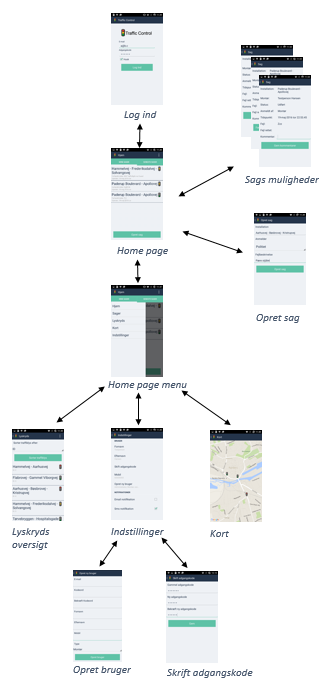
\includegraphics[scale=1.6]{Android/Billeder/Navigation}
		\end{center}
		\caption{Sekvens diagram for log ind på android applikationen}
		\label{fig:Navigation i applikationen}
	\end{figure}
	\pagebreak
	
	\section{Design og Implementering} \label{sec:designandroid}
	Denne sektion indeholder en uddybende forklaring af design og implementering.
	Der er brugt MVP design pattern til alle activities, samt dependency injection for at gøre koden testbar og åben for udvidelser. BLL-laget anvender en factory til at oprette Model objekter. Det er gjort fordi, GUI-laget ikke skal kende til DAL-laget. Hvis en model har en dependency i DAL-laget, bliver denne oprettet i den factory som ligger i BLL-laget.
	
	
	\subsection{Log ind}
	Dette afsnit vil indeholde en gennem gang af design, grafisk bruger interface og implementering af Log ind activity til android applikationen
	
	\clearpage
	
	\subsubsection{Design}
	På figur \ref{fig:Sekvens diagram for Log Ind Android} ses et sekvens diagram over log ind forløbet til android applikationen
	\begin{figure} [!ht]
		\begin{center}
			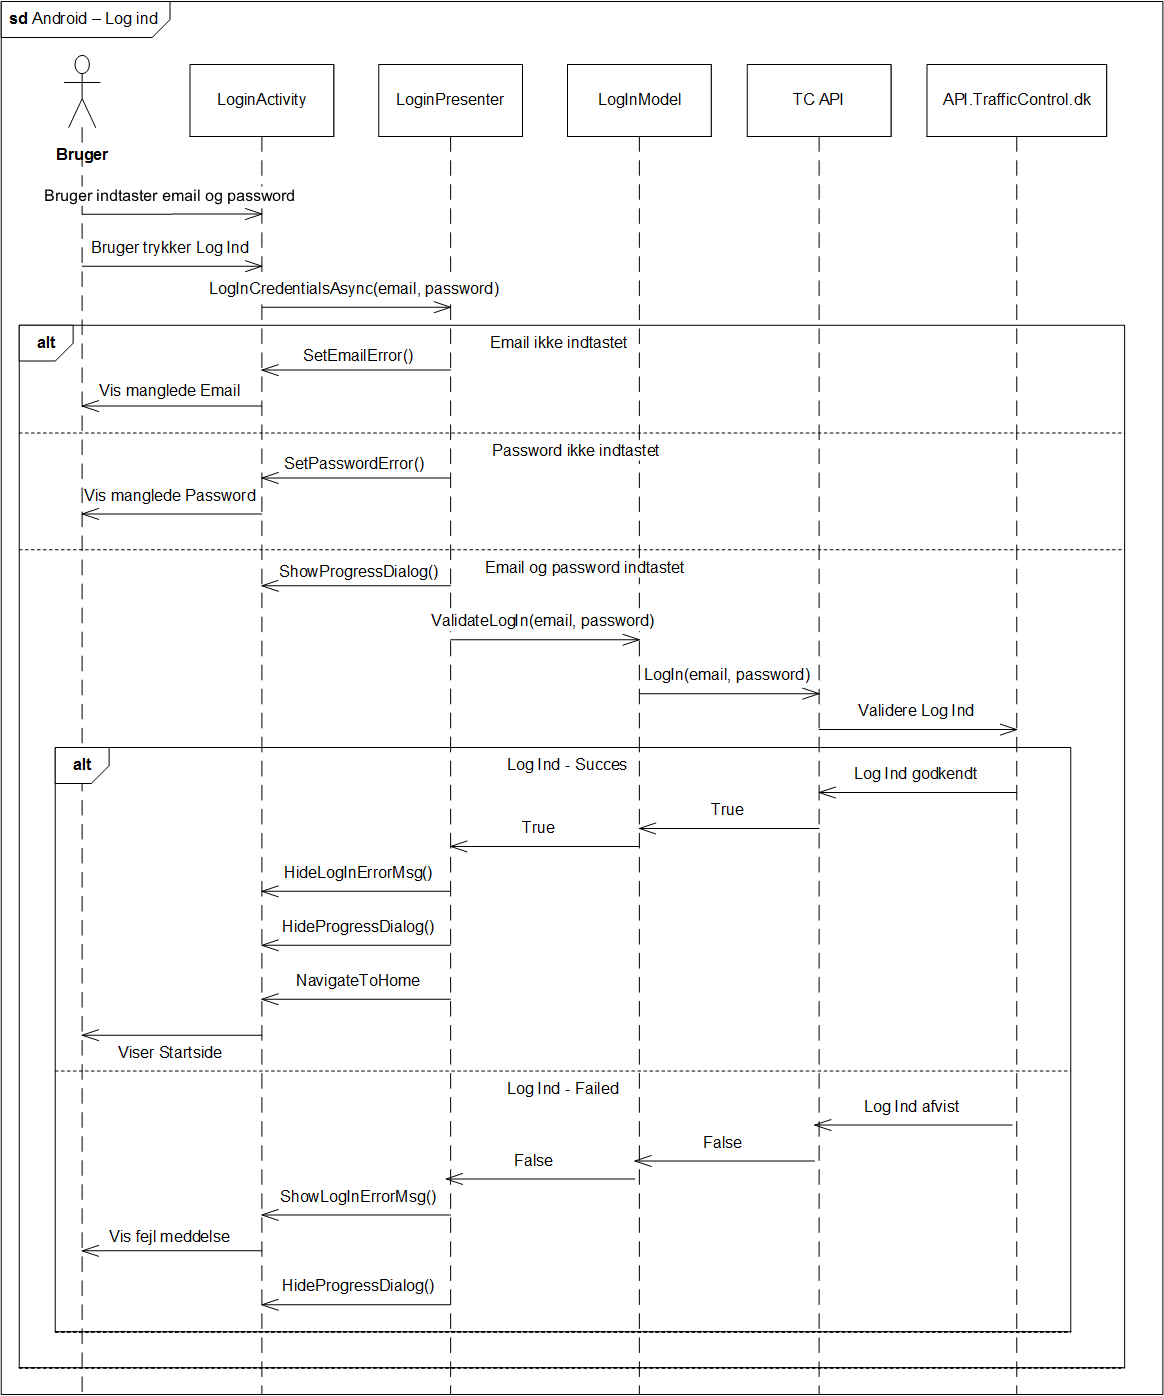
\includegraphics[width=1\textwidth]{Android/Billeder/SekvensDiagramLogInd}
		\end{center}
		\caption{Sekvens diagram for log ind på Android applikationen}
		\label{fig:Sekvens diagram for Log Ind Android}
	\end{figure}
	
	\clearpage
	
	På figur \ref{fig:Klasse diagram for Log Ind Android} ses hvordan klasserelationerne til Login activity er designet, med udgangspunkt i MVP.
	
	\begin{figure} [!ht]
		\begin{center}
			\includegraphics[width=0.8\textwidth]{Android/Billeder/clLogin}
		\end{center}
		\caption{Klasse diagram for log ind på Android applikationen}
		\label{fig:Klasse diagram for Log Ind Android}
	\end{figure}
	
	\clearpage
		
	\subsubsection{Grafisk Brugergrænseflade}
	På figur \ref{fig:Traffic Control - Log ind} ses hvordan at Log Ind siden ser ud på android applikationen.
	Det er et meget simpelt design, for at gøre det yderst bruger venligt.
	
	\begin{figure} [h]
		\begin{center}
			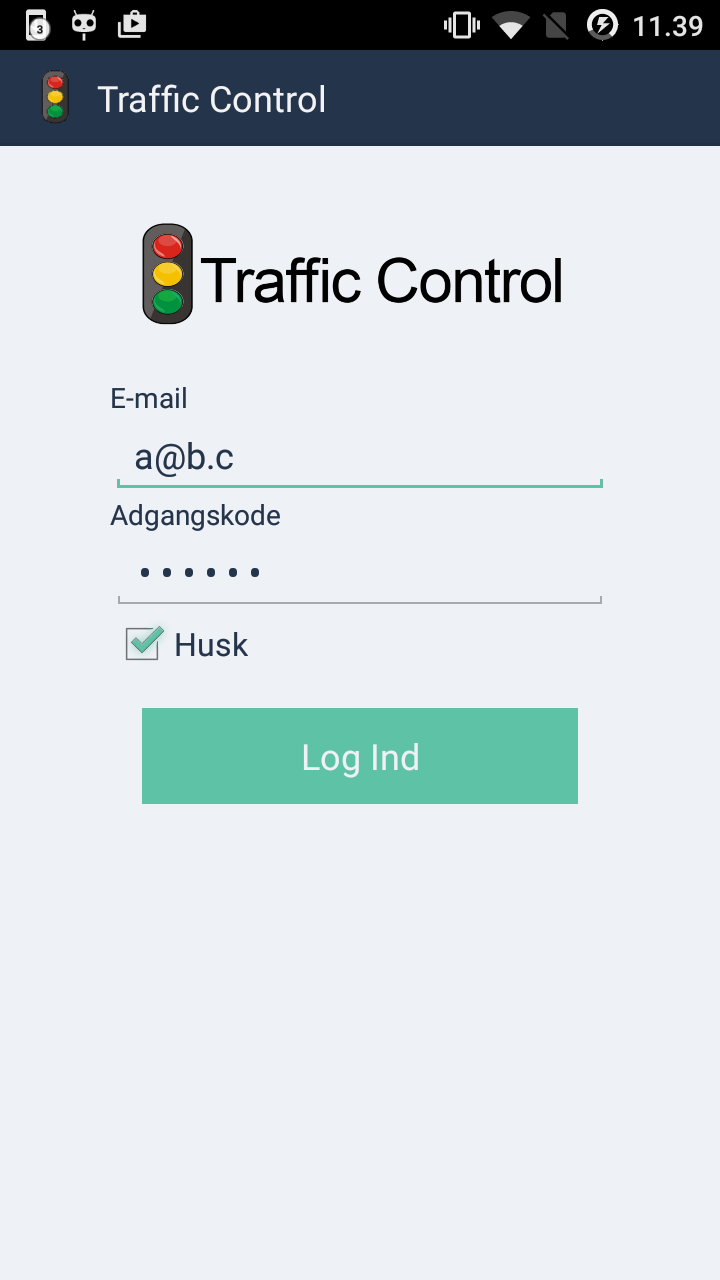
\includegraphics[height=7cm]{Android/Billeder/AndroidLogIn}
		\end{center}
		\caption{Traffic Control - Log ind}
		\label{fig:Traffic Control - Log ind}
	\end{figure}
	
	\subsubsection{Implementering}
	Når en bruger forsøger at logge ind, validerer presenteren at der er indtastet information, inden at informationen bliver sendt videre til modellen. Hvis et felt ikke er udfyldt giver presenteren en fejlbesked til viewet. Hvis alle de påkrævede felter er fyldt ud bliver et request sendt til API'et, gennem Modellen og DAL-laget. 
	\\Specielt for LogInActivity, benyttes en privat fil på telefonen til at gemme log ind oplysninger. Ansvaret for sikkerheden af denne fil, står Android frameworket for.
	
	\pagebreak
	\subsection{Home page}
	Dette afsnit vil indeholde en gennem gang af design, grafisk bruger interface og implementering af Homeactivity til android applikationen
	\subsubsection{Design}
	HomeActivity er bygget op om samme design som LogIn, der er dog tilføjet et fragment for hver af de to tabs i layoutet. Fragmentet opfører sig som en selvstændig activity, som lever i HomeActivity. 
	\\HomeActivity bruger interfacet IUserPreference til at hente bruger oplysninger ned, og gemme dem.
	\\Strukturen af HomeActivity kan ses på figur \ref{fig:Klasse diagram for HomeActivity}
	\begin{figure}[h!]
		\begin{center}
			\includegraphics[height=8cm]{Android/Billeder/clHomeActivity}
		\end{center}
		\caption{Fragment struktur for HomeActivity}
		\label{fig:Klasse diagram for HomeActivity}
	\end{figure}
	\pagebreak
	
	\subsubsection{Grafisk Brugergrænseflade}
	Hjemsiden er mere kompleks end de andre sider. Dette simplificeres ved ikke at vise mange egenskaber af gangen. Se layout på figur \ref{fig: Traffic Control - Home Page}
	\begin{figure}[h!]
		\begin{center}
			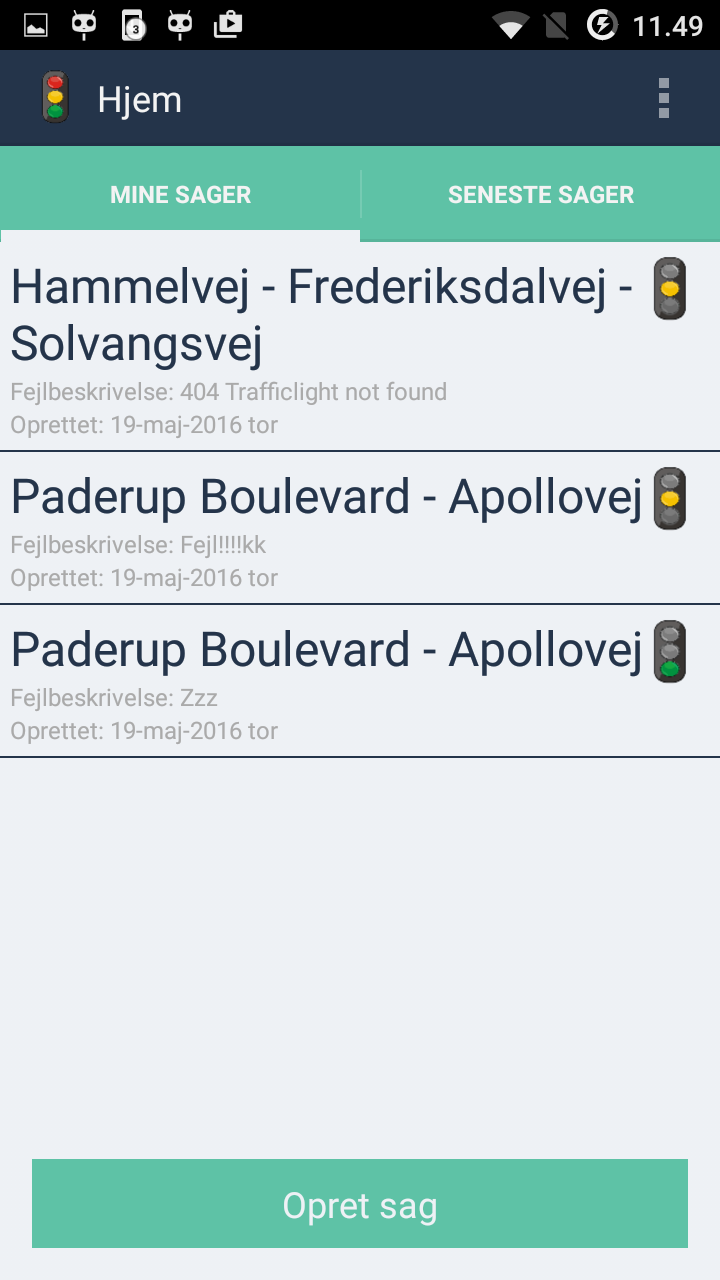
\includegraphics[height=8cm]{Android/Billeder/AndroidHomePage}
		\end{center}
		\caption{Traffic Control - Home Page}
		\label{fig: Traffic Control - Home Page}
	\end{figure}
	\\
Hjemsiden indeholder en liste af sager. Trafiklysikonet ud for sagen viser hvilken status sagen er i.
\begin{itemize}
	\item \textbf{Rød} når en sag er oprettet, men ikke taget af en montør endnu
	\item \textbf{Gul} når en montør har taget sagen, og påbegyndt arbejde på den
	\item \textbf{Grøn} når sagen er færdig og ikke kan genåbnes igen
\end{itemize}
Der er to tabs hvor man enten kan vælge at se alle sager eller se de sager brugeren selv har taget.
\\Der kan findes en menu, hvis der swipes fra venstre mod højre, hvor navigation til resten af applikationen kan foretages.
	
	
	\subsubsection{Implementering}\label{HomePageImp}
	HomeActivity er også bygget op omkring MVP, hvor sager bliver gemt i modellen. Modellen indeholder de sager der er tilknyttet brugeren som er logget ind, samt de seneste 1000 sager. Alt data hentes fra DAL-laget.
	\\For at kunne vise "Mine sager" og "Alle sager" på en fornuftig måde, består HomeActivity af to fragmenter. Som hver især har en presenter og en model, altså samme design som LogInActivity på figur \ref{fig:Klasse diagram for Log Ind Android}.
	\\Der er lavet en Drawer menu i venstre side, til navigation af applikationen. Funktionallitet og layout til menuen er lavet i klassen MenuActivity, som HomeActivity nedarver fra, og derved har HomeActivity menu funktionallitet.
	Et klassediagram for dette, kan ses på figur \ref{fig:Klasse diagram for HomeActivity}.
	 
	\pagebreak
	
	\subsection{Opret bruger}
	Dette afsnit vil indeholde en gennem gang af design, grafisk bruger interface og implementering af Opret bruger activity til android applikationen
	\subsubsection{Design}
	På figur \ref{fig:OpretBrugerSekvens} vises et sekvens diagram over Opret bruger forløbet i android applikationen
	
	\begin{figure} [!ht]
		\begin{center}
			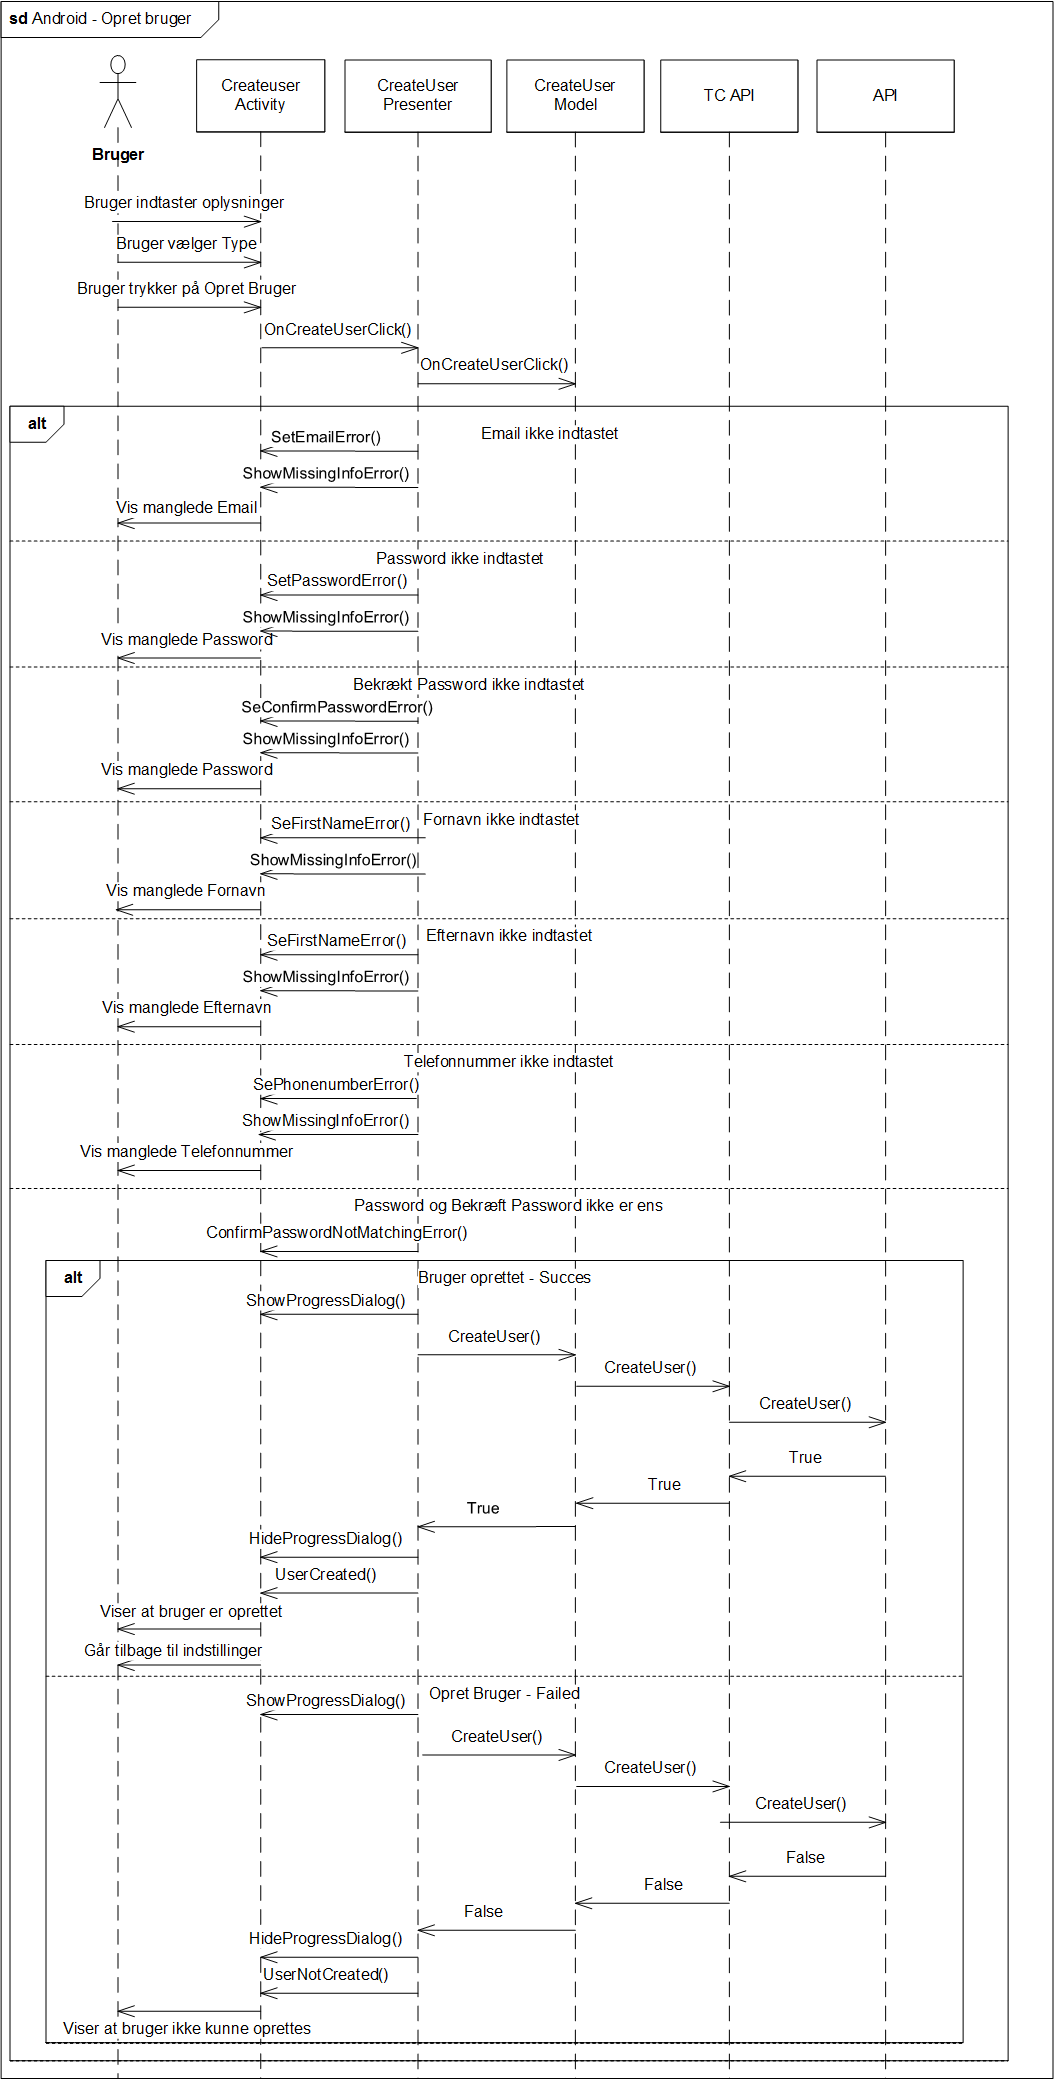
\includegraphics[height=15cm, width=11cm]{Android/Billeder/OpretBrugerSekvens}
		\end{center}
		\caption{Sekvens diagram for opret bruger på android applikationen}
		\label{fig:OpretBrugerSekvens}
	\end{figure}
	Klasse relationerne svarer overens men dem i LogInActivity på figur \ref{fig:Klasse diagram for Log Ind Android}. Da opret bruger siden er bygget op omkring MVP på samme måde som log ind siden.
	
	\clearpage
	
	\subsubsection{Grafisk Brugergrænseflade}
	På Opret bruger siden er der lavet felter til alt det info som skal tastes ind om en bruger og til sidst er der lavet en drop down hvor du kan vælge hvilken type bruger det er.
	Se figur \ref{fig: Traffic Control - Opret Bruger}.
	
	\begin{figure}[!ht]
		\begin{center}
			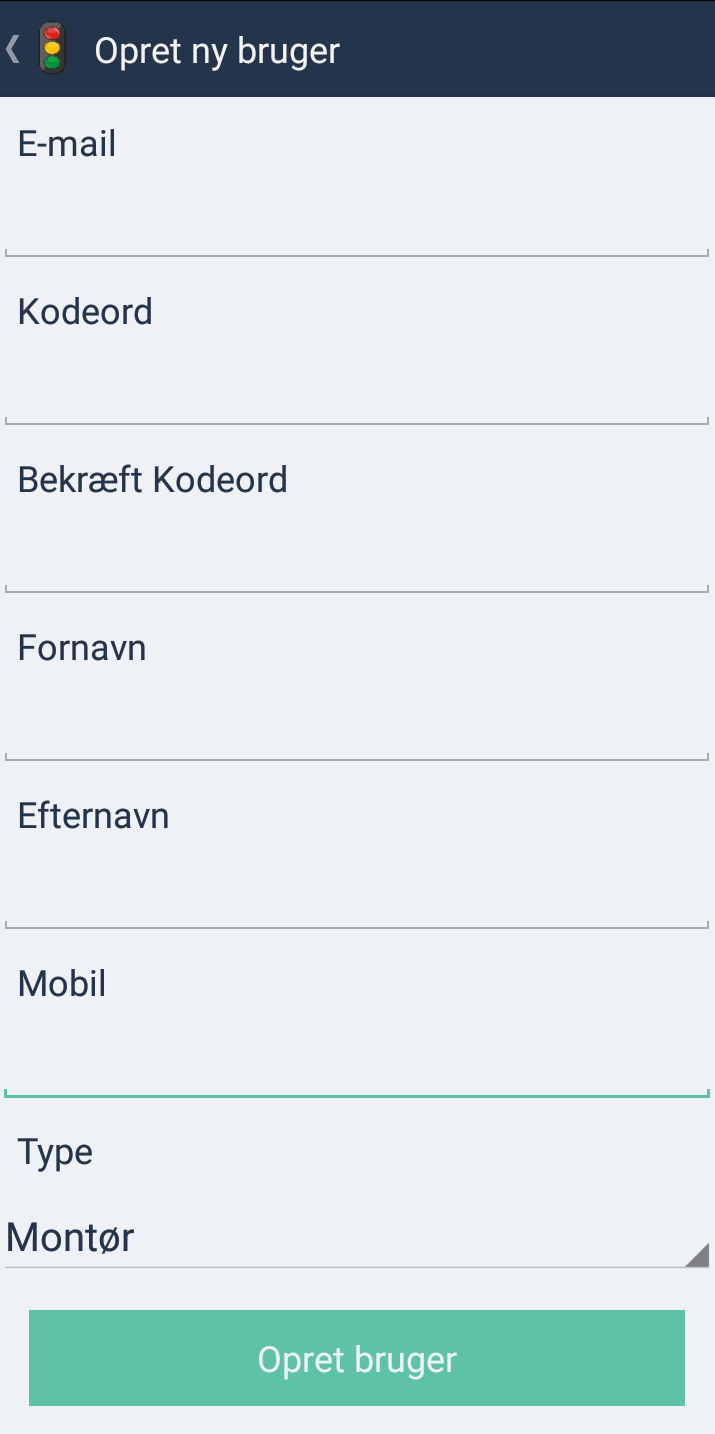
\includegraphics[height=9cm]{Android/Billeder/AndroidOpretbruger}
		\end{center}
		\caption{Traffic Control - Opret Bruger}
		\label{fig: Traffic Control - Opret Bruger}
	\end{figure}
	 	
	\subsubsection{Implementering}
	Når der skal oprettes en ny bruger, validerer presenteren at der er indtastet information, inden at informationen bliver sendt videre til modellen. Hvis et felt ikke er udfyldt giver presenteren fejlbesked til viewet. Hvis alle de påkrævede felter er fyldt ud bliver et request sendt til API'et, gennem Modellen og DAL.	
	\pagebreak
	
	
	\subsection{Opret sag}
	Dette afsnit vil indeholde en gennem gang af design, grafisk bruger interface og implementering af Opret sag activity til android applikationen
	\subsubsection{Design}
	Opret sag er designet efter samme fremgangsmåde som opret bruger. Det kan ses på figur \ref{fig:OpretBrugerSekvens}. Hvor input felterne bliver valideret, og udfra dette gives der feedback til brugeren om eventuelle fejl. 
	Klasse relationerne er bygget op på samme måde som opret bruger og log ind, som kan ses på figur \ref{fig:Klasse diagram for Log Ind Android}.
	Dog med andre navne tilsvarende opret sag activity.
	
	\subsubsection{Grafisk Brugergrænseflade}
	På figur \ref{fig:Opret sag på android applikationen } ses layout af Opret sag på android applikationen.
	\begin{figure} [!ht]
		\begin{center}
			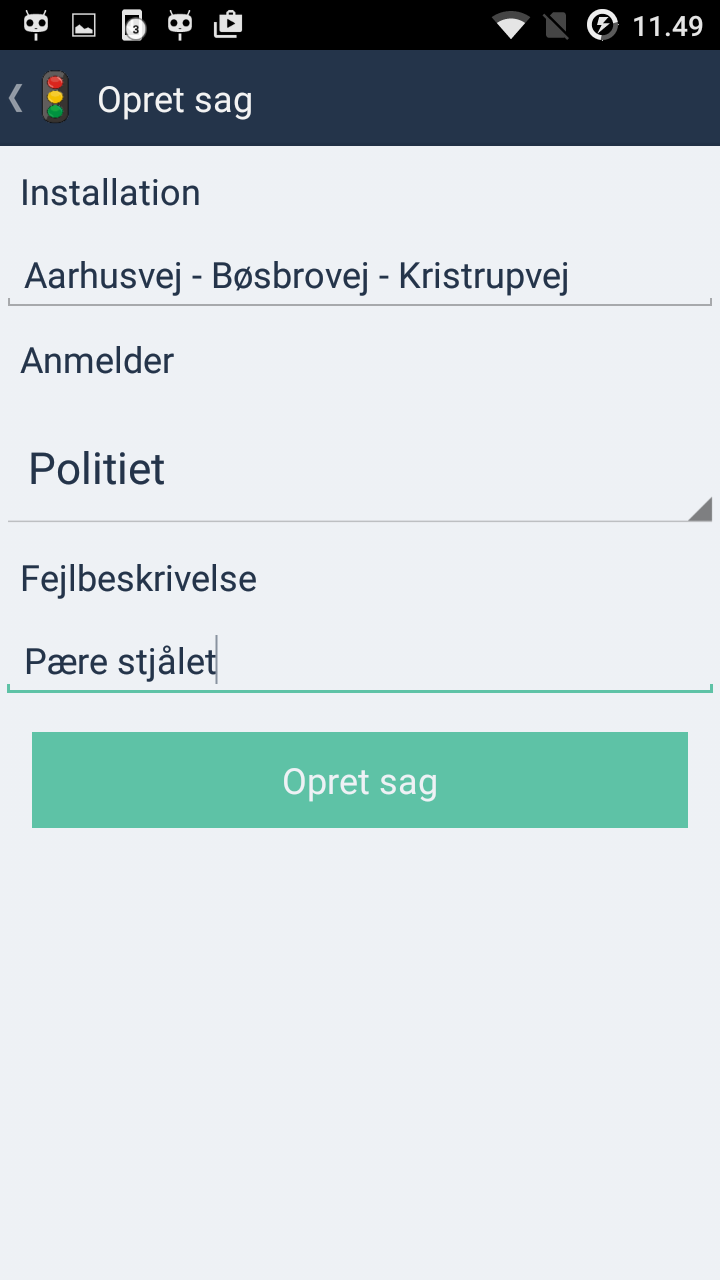
\includegraphics[height=10cm]{Android/Billeder/AndroidOpretSag}
		\end{center}
		\caption{Sekvens diagram for lyskryds oversigt på android appliktionen}
		\label{fig:Opret sag på android applikationen }
	\end{figure}
	
	\subsubsection{Implementering}
	Når der skal oprettes en ny sag, validerer presenteren at der er indtastet information, inden at informationen bliver sendt videre til modellen. Hvis et felt ikke er udfyldt giver presenteren fejlbesked til viewet. Hvis alle de påkrævede felter er fyldt ud bliver et request sendt til API'et, gennem Modellen og DAL-laget.
	\\Der er implementeret autocomplete på feltet "Installation", som henter sine forslag for modellen. På samme måde hentes valgmuligheder til feltet "Anmelder" også fra modellen.
	\pagebreak
	
	
	\subsection{Sag}
	Dette afsnit vil indeholde en gennem gang af design, grafisk bruger interface og implementering af Vis sag activity til android applikationen
	\subsubsection{Design}
	Vis sag activity er bygget op på samme måde som bl.a. LogInActivity, ud fra MVP. Et klasse diagram for dette kan ses på figur \ref{fig:Klasse diagram for Log Ind Android}.
	Specielt for design af CaseActivity, er der lavet flere forskellige layout som skal vises afhængigt af hvilken status den valgte sag har. Sekvensen for dette kan ses på figur \ref{fig:Sekvensdiagram CaseActivity}.
	
	\begin{figure} [!ht]
		\begin{center}
			\includegraphics[height=10cm]{Android/Billeder/sdCaseActivity}
		\end{center}
		\caption{Sekvensdiagram for layout selection}
		\label{fig:Sekvensdiagram CaseActivity}
	\end{figure}
	
	\clearpage
	
	\subsubsection{Grafisk Brugergrænseflade}
	De forskellige layouts til at vise en sag ses nedenfor.\\	
	På figur \ref{fig:Sag der ikke er taget på android applikationen} ses der en sag som ikke er taget.
	Figur \ref{fig:Sag der er taget på android applikationen} viser en sag som er taget af en montør.
	På den sidste figur \ref{fig:Sag der er faerdig på android applikationen} ses en sag der er færdig behandlet.
	
	\begin{figure} [!ht]
		\begin{center}
			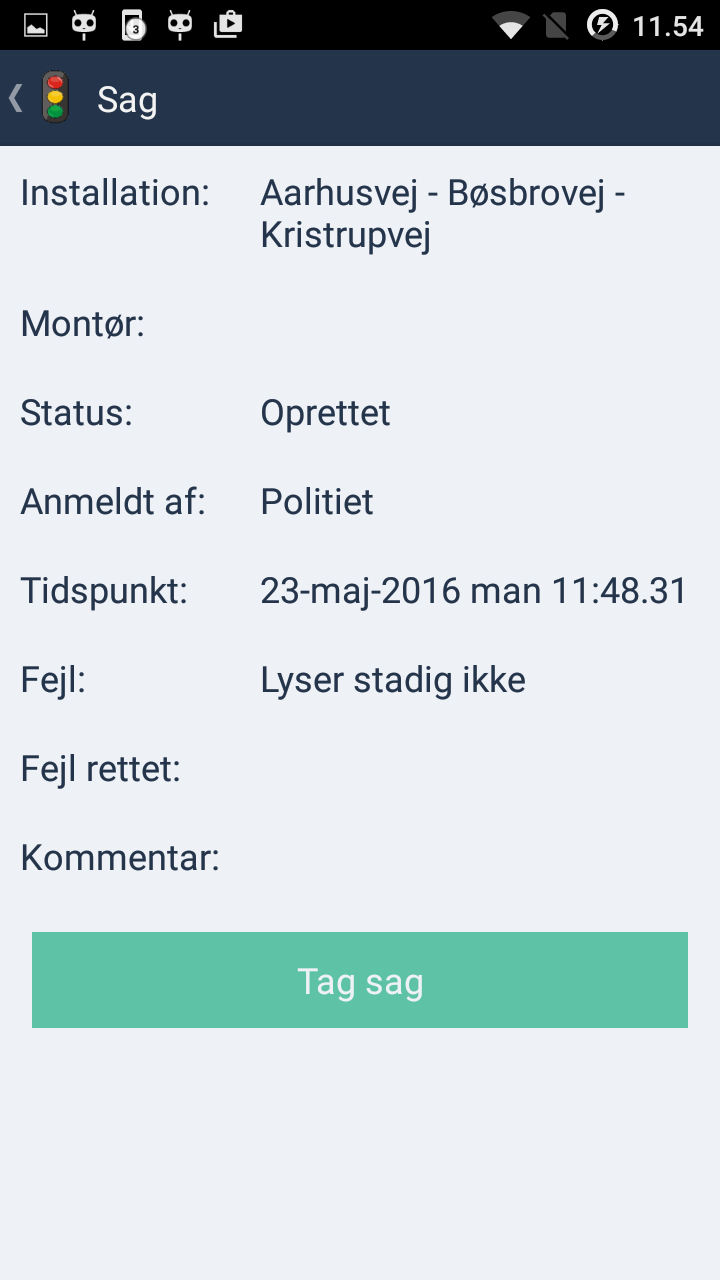
\includegraphics[height=10cm]{Android/Billeder/AndroidSagRod}
		\end{center}
		\caption{Sag der ikke er taget på android applikationen}
		\label{fig:Sag der ikke er taget på android applikationen}
	\end{figure}
	
	\newpage
	
	\begin{figure} [!ht]
		\begin{center}
			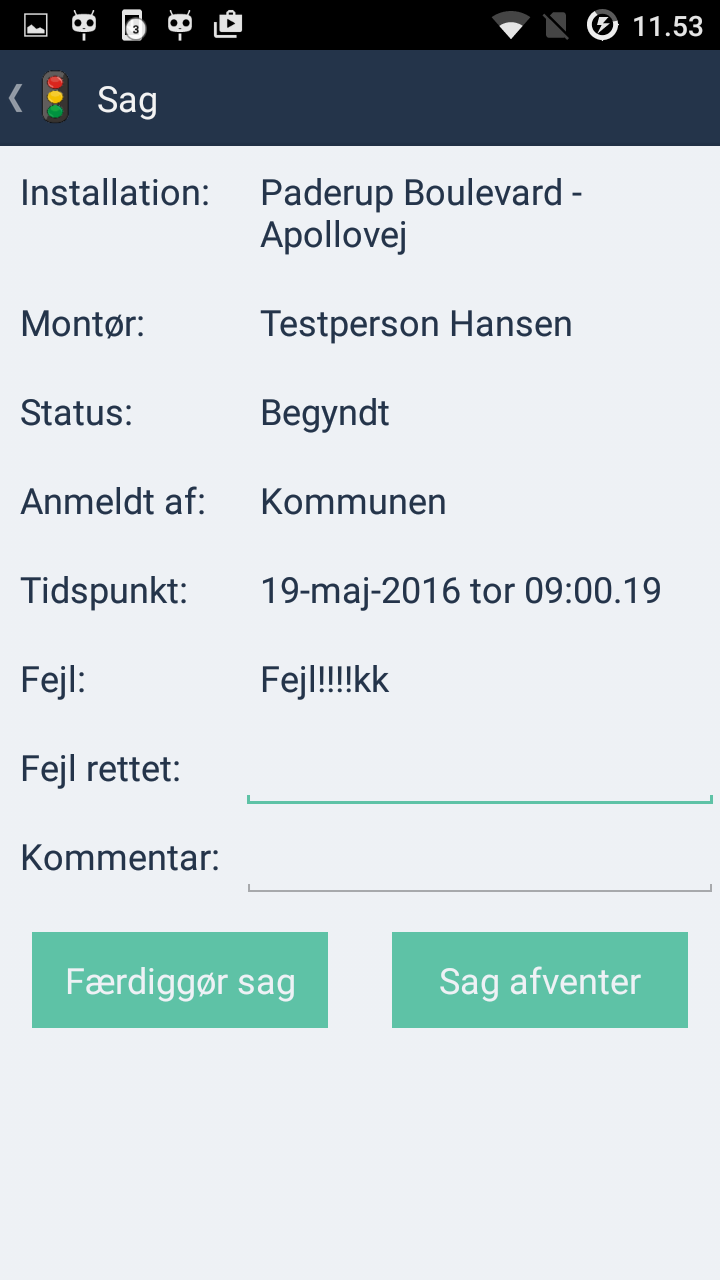
\includegraphics[height=8cm]{Android/Billeder/AndroidSagGul}
		\end{center}
		\caption{Sag der er taget på android applikationen}
		\label{fig:Sag der er taget på android applikationen}
	\end{figure}
	
	\begin{figure} [!ht]
		\begin{center}
			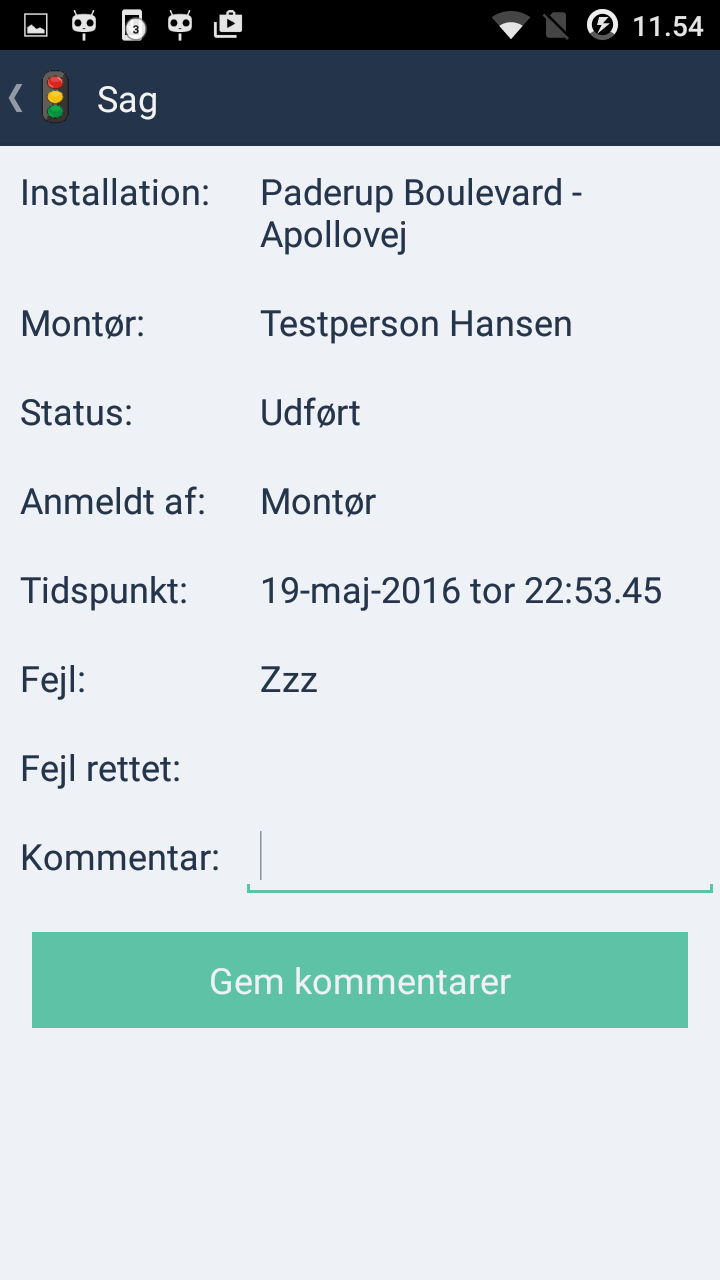
\includegraphics[height=8cm]{Android/Billeder/AndroidSagGron}
		\end{center}
		\caption{Sag der er færdig på android applikationen}
		\label{fig:Sag der er faerdig på android applikationen}
	\end{figure}
	
	\subsubsection{Implementering}
	For hvert layout, har presenteren en funktion som bestemmer hvad der skal ske når en pågældende knap i layoutet bliver trykket på. Den valgte sag bliver opdateret med ny status, kommentarer og andet information. Derefter sendes sagen til modellen som sørger for at sagen bliver opdateret i databasen via DAL-laget og API.
	\\Hvis en sag ikke kunne opdateres, giver presenteren viewet besked om at der skal vises en fejlmeddelelse. 
			
	\clearpage		
	
	\subsection{Kort}
		Dette afsnit vil indeholde en gennem gang af design, grafisk bruger interface og implementering af Kort activity til android applikationen
	\subsubsection{Design}
	Der er brugt samme design mønster til MapActivity som til, de andre activities, et eksempel på dette design kan findes på figur \ref{fig:Klasse diagram for Log Ind Android}.
	\\Specielt til kortet, er der lavet en factory som sender en reference til de ikoner (bitmaps) som skal vises på kortet. På den måde allokeres der ikke 100 ens ikoner i hukommelsen på telefonen, hvis kortet skal vise 100 små lyskryds.

	\subsubsection{Grafisk Brugergrænseflade}
	Nedenfor, på figur \ref{fig:Map på android appliakationen}, ses hvordan kortet viser små ikoner af lyskryds. Farven på lyskrydset indikerer hvilken status det er i. Rød betyder at der er en ny sag på lyskrydset, som der ikke er taget endnu. Gul betyder at sagen er taget og bliver behandlet. Grøn betyder at der ikke er en sag på lyskrydset, eller at alle sager er færdiggjort.
	\begin{figure} [!ht]
		\begin{center}
			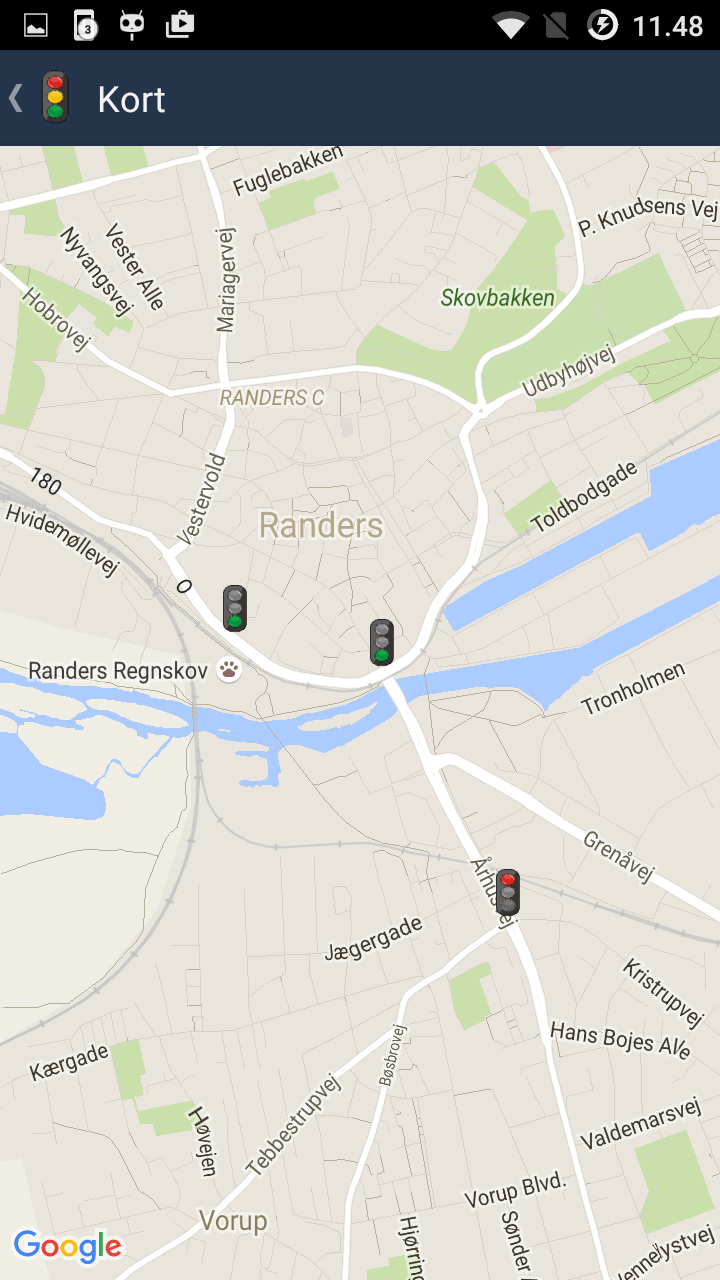
\includegraphics[height=10cm]{Android/Billeder/AndroidMap}
		\end{center}
		\caption{Map på android appliakationen}
		\label{fig:Map på android appliakationen}
	\end{figure}
	
	\clearpage
		
	\subsubsection{Implementering}
	Til implementering af et kort i android applikationen, er der brugt Googles Map Api\cite{GoogleMapApi}. Når et map oprettes kan det godt tage forholdsvis lang tid at hente mappet fra Api'et. Derfor er der lavet et callback, som bliver kaldt når mappet er hentet færdigt. I det callback ligger al funktionaliteten til, at tilføje ikoner, og zoome ind på de rigtige koordinater der skal vises.
	\\Positionerne på de ikoner der bliver vist, hentes gennem TrafficControl Api.\\
	
\subsection{Lyskryds oversigt}
Dette afsnit vil indeholde en gennemgang af design, grafisk bruger interface og implementering af Lyskryds oversigt activity til android applikationen.
\subsubsection{Design}
På figur \ref{fig:Design over lyskryds oversigten på android applikationen} ses et design over Lyskryds oversigt activity til android applikationen.
\begin{figure} [!ht]
	\begin{center}
		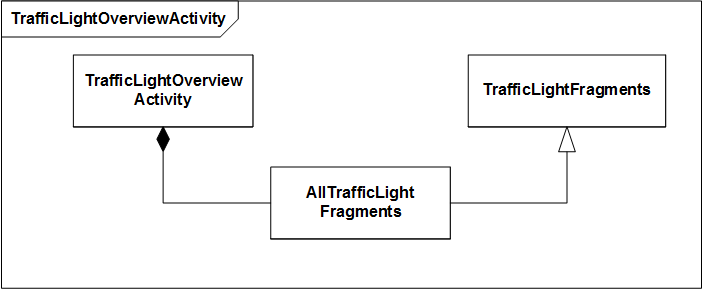
\includegraphics[height=7cm]{Android/Billeder/Lyskryds}
	\end{center}
	\caption{Design over lyskryds oversigten på android applikationen}
	\label{fig:Design over lyskryds oversigten på android applikationen}
\end{figure}\\
TrafficLightOverviewActivity er bygget op om samme design som HomeActivity, se figur \vref{fig: Traffic Control - Home Page}. TrafficLightOverviewActivity har fået tilføjet et felt hvor du kan vælge en værdi du ønsker at sortere lyskrydsene efter.

\pagebreak

\subsubsection{Grafisk Brugergrænseflade}
Her vises layouttet af Lyskryds Oversigt activity på android applikationen.\\	
\begin{figure} [!ht]
	\begin{center}
		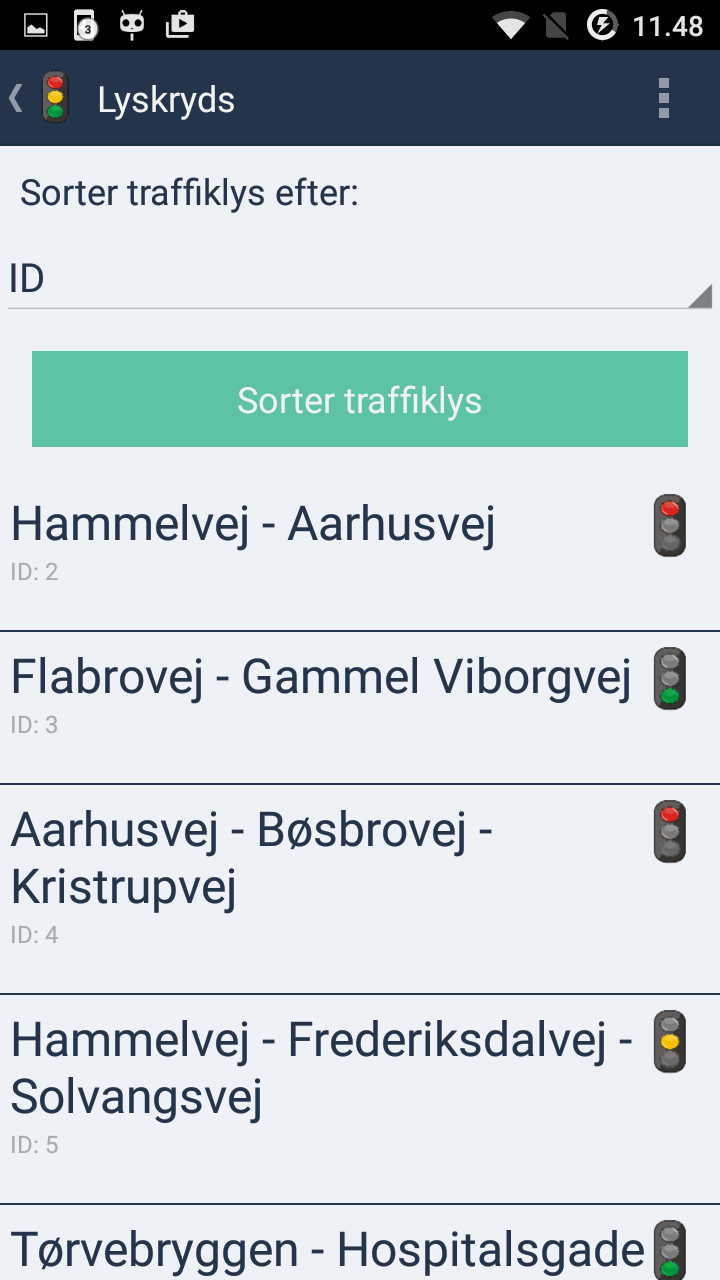
\includegraphics[height=10cm]{Android/Billeder/AndroidLyskryds}
	\end{center}
	\caption{Oversigt over lyskryds på android applikationen}
	\label{fig:Oversigt over lyskryds på android applikationen}
\end{figure}

\noindent Denne activity i applikationen bruges til at få et overblik over alle lyskryds i databasen. Man kan sortere alle lyskryds efter; adresse, ID eller status. Man kan se status på et lyskryds ud fra ikonet. Ikonet viser rød eller gul, hvis der er en sag der skal have opmærksomhed. Hvis lyskrydset ingen sager har viser ikonet grøn.\\
Her fra vil man kunne navigere videre til de enkelte lyskryds, hvorfra man kan se lyskrydsets status, placering, log og bilag.

\subsubsection{Implementering}
Modellen indeholder alle de lyskryds der er i Randers kommune, disse hentes fra DAL-laget.
Der er øverst i TrafficLightOverviewActivity lavet en spinner samt en knap som gør det muligt at vælge en værdi som ønskes lyskryds sorteret efter.
Sorterings delen består af to fragments som i Homeactivity, se afsnit \vref{HomePageImp}.


\pagebreak 
	
	
	\subsection{Indstillinger}
	Dette afsnit vil indeholde en gennemgang af design, grafisk bruger interface og implementering af Indstillinger activity til android applikationen.
	\subsubsection{Design}
	Der er brugt samme design mønster til SettingsActivity som til, de andre activities, et eksempel på dette design kan findes på figur \ref{fig:Klasse diagram for Log Ind Android}.
	
	\subsubsection{Grafisk Brugergrænseflade}
	På figur \ref{fig:Instillinger på android applikationen} ses layout for Indstillinger på android applikationen.	
	\begin{figure} [!ht]
		\begin{center}
			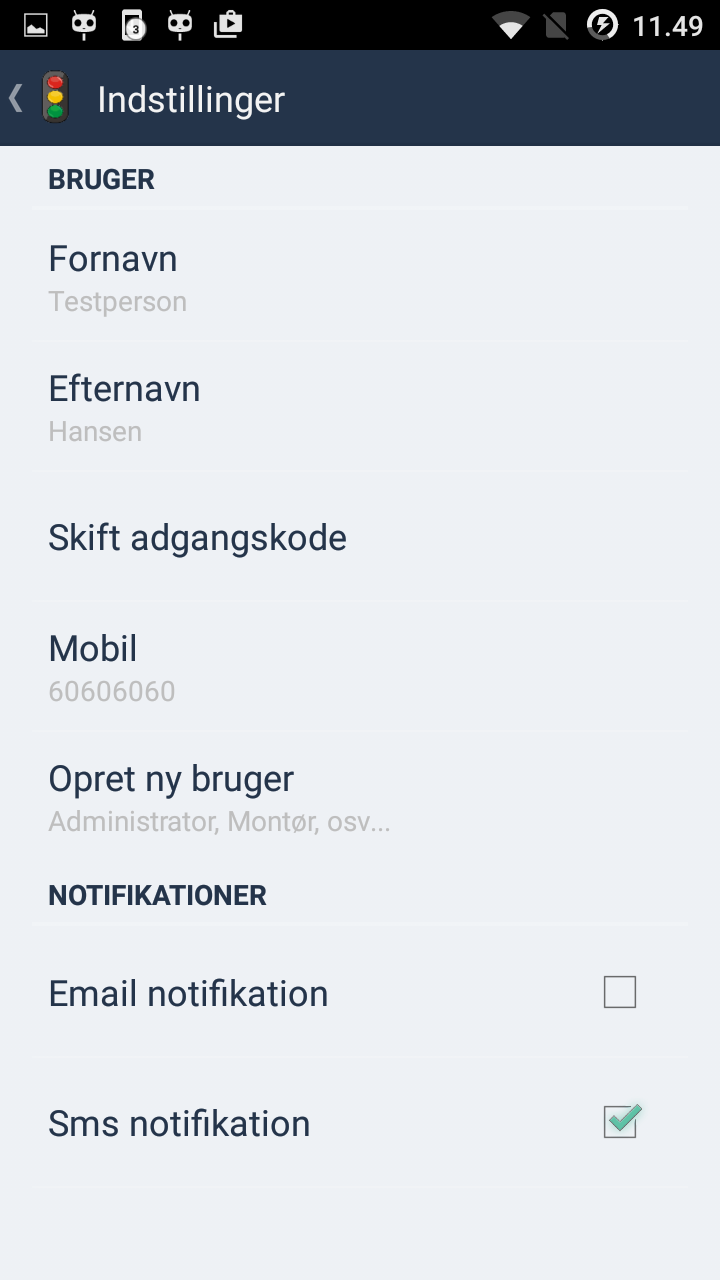
\includegraphics[height=10cm]{Android/Billeder/AndroidInstillinger}
		\end{center}
		\caption{Indstillinger på android applikationen}
		\label{fig:Instillinger på android applikationen}
	\end{figure}
	
	\subsubsection{Implementering}
	Til implementeringen af SettingsActivity, er der tilføjet et SettingsFragment, som nedarver fra PreferenceFragment. PreferenceFragment er en klasse fra Xamarin.Android Api'et \cite{XamarinDoc}, som har en funktion der kaldes når en Preference ændres. 
	\\Preferences i Android svarer til indstillinger. Når en indstilling ændres, kaldes Api'et med ændringen. Indstillinger ligger også gemt lokalt på telefonen i en privat fil, og bliver opdateret sammen med kaldet til Api'et.
	
	\clearpage
	
	\subsection{Skift adgangskode}
		Dette afsnit vil indeholde en gennemgang af design, grafisk bruger interface og implementering af Skift adgangskode activity til android applikationen.
	\subsubsection{Design}
	Skift adgangskode er designet efter samme fremgangsmåde som opret bruger. Det kan ses på figur \ref{fig:OpretBrugerSekvens}, hvor input felterne bliver valideret, og udfra dette gives der feedback til brugeren om eventuelle fejl. 
	
	\subsubsection{Grafisk Brugergrænseflade}
	Layout for at skifte adgangskode på brugeren som er logget ind, kan ses på figur \ref{fig:Skift adgangskode på android applikationen}.	
	\begin{figure} [!ht]
		\begin{center}
			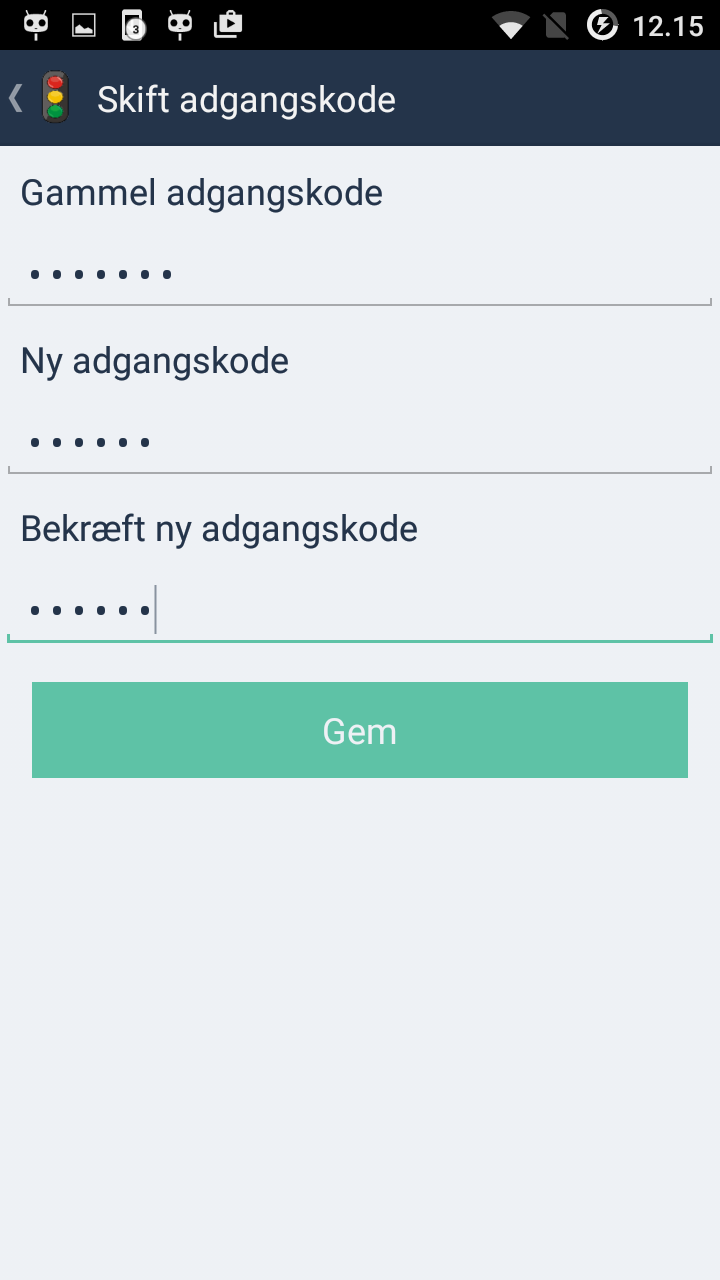
\includegraphics[height=10cm]{Android/Billeder/AndroidSkiftAdgangskode}
		\end{center}
		\caption{Skift adgangskode på android applikationen}
		\label{fig:Skift adgangskode på android applikationen}
	\end{figure}
	
	\subsubsection{Implementering}
	Når en bruger forsøger at skifte adgangskode, validerer presenteren at der er indtastet information. Hvis den nye adgangskode passer overens med den bekræftede kode, bliver informationen sendt videre til modellen. Hvis et felt ikke er udfyldt giver presenteren fejlbesked til viewet. Hvis alle de påkrævet felter er fyldt ud bliver et request sendt til API'et, gennem Modellen og DAL-laget.
	
	\pagebreak
	
	\section{Test}
	I dette afsnit beskrives hvordan android applikationen er testet. For yderligere information omkring tests, henvises der til source koden tilhørende android applikationen.
	\\	For at gøre android applikationen testbar, er der brugt MVP design pattern og dependency injection i klasserne. Dette muliggør at afhængigheder kan mockes ud. 
	
		\begin{figure} [!ht]
			\begin{center}
				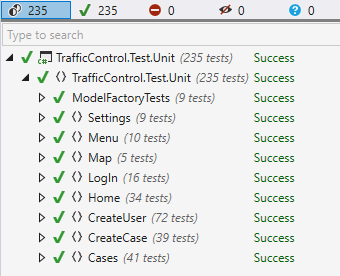
\includegraphics[height=7cm,width=12cm]{Android/Billeder/AndroidTests}
			\end{center}
			\caption{Oversigt over unittests udført på Android Applikationen}
			\label{fig:AndroidTests}
		\end{figure}
		
	På overstående figur \ref{fig:AndroidTests}, ses de unittests som er udført på android applikationen. Der er ikke lavet tests af views, da test frameworket ikke understøtter android biblioteker.

	Et eksempel på en unittest ses på figur \ref{fig:AndroidUnitTestEksempel}. Det er en test for CasePresenter, og der testes om den nuværende sags information bliver gemt korrekt, når PendingCase kaldes.
	
	\begin{figure} [!ht]
		\begin{center}
			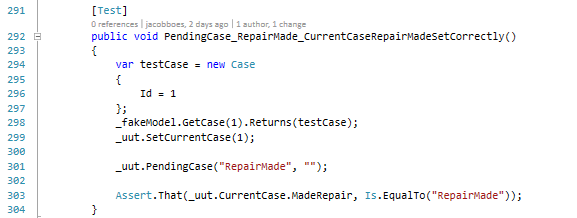
\includegraphics[height=7cm,width=17cm]{Android/Billeder/unittestEksempel}
		\end{center}
		\caption{Eksempel på en unittest på Android Applikationen}
		\label{fig:AndroidUnitTestEksempel}
	\end{figure}
			
	